\chapter{Software}

The software of the speaker has two main goals: Controlling the movement and playing an audio signal from an external source over SPI. Because both parts of the software don't need to interact with each other it was decided to split them up into two separate programs. The Speaker control is written in python but the Sound playback is written in C++ to increase performance.\p
%
A Raspberry Pi 3 Model B+ was chosen to run the software. With its Linux operating system it provides an easy way to parallize tasks. The Raspberry Pi also has a SPI interface and enough PWM pins to control the Servo Motors.\cite{van_loo_bcm2836_2014}

\section{Sound Playback}

The sound playback program starts by reading samples from a connected audio device. Those samples are then modulated and sent over SPI with the right sampling rate. In order to generate a fluent audio playback the tasks where splitted into three threads. The whole sequence of the program is shown in figure \ref{fig:software:sound_sequence}.\p
%
Reading audio samples and modulating them is done in the class \lstcpp{AudioProcessor}. The SPI transmission is handled in the class \lstcpp{Speaker}. Both classes are built with the singleton pattern.
%
\begin{figure}
  \centering
  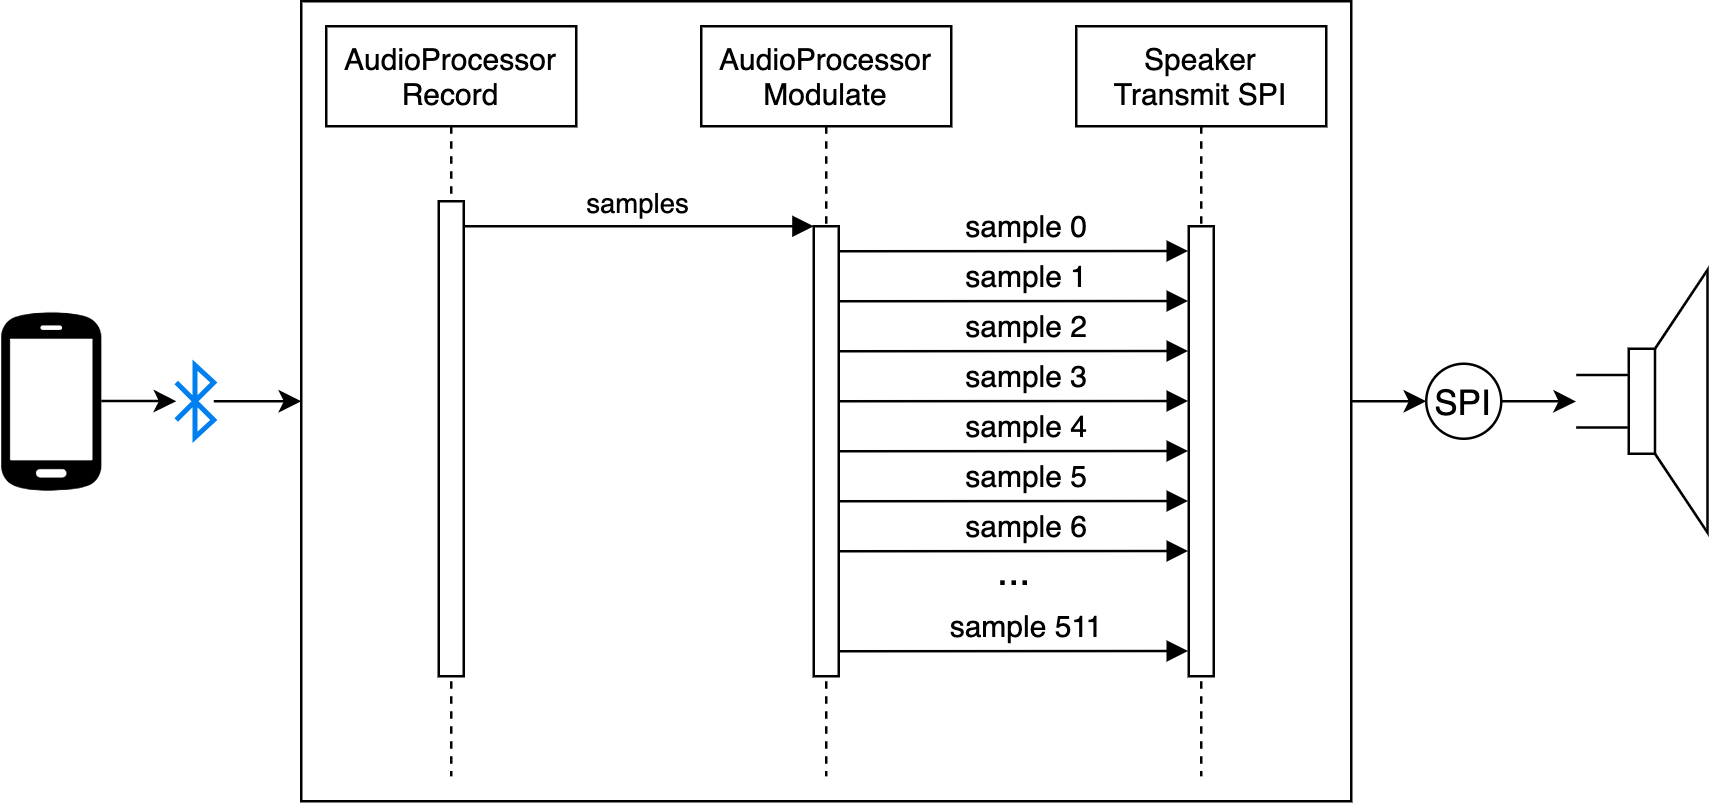
\includegraphics[width=\textwidth]{src/assets/pictures/software/sequence_diagramm.png}
  \caption{Sound playback sequence diagram}\label{fig:software:sound_sequence}
\end{figure}
\p
The communication between threads is handlend with a queue. The implementation shown in listing \ref{lst:software:queue} makes the \lstcpp{std::queue} threadsafe by using a lock to access the underlying queue and also blocks the thread if no data is available. This is usefull, among other things, because there is no need to send data over SPI when no new sample is generated.\p
%
A hardware abstraction layer is used to separate logic and hardware interfaces.
%
\begin{mdframed}
\begin{lstlisting}[caption=Threadsafe and blocking queue, label=lst:software:queue]
template <class T> class BlockingQueue : public queue<T> {
  public:
  void push(T item) {
    {
      unique_lock<std::mutex> lck(lock);
      queue<T>::push(item);
    }
    not_empty.notify_one();
  }

  T pop() {
    unique_lock<std::mutex> lck(lock);
    not_empty.wait(lck, [this]() { return queue<T>::size() > 0; });

    T value = queue<T>::front();
    queue<T>::pop();
    return value;
  }

  bool notEmpty() { return !queue<T>::empty(); }

  private:
  std::mutex lock;
  condition_variable not_empty;
};
\end{lstlisting}
\end{mdframed}

\subsection{Audio input}\label{sec:software:rec}
%
There are different methods to connect an external audio device to the Raspberry Pi. The Raspberry provides an AUX port where the microphone line could be used as input. An alternative would be to use an external USB audio card or a audio card HAT with a dedicated AUX IN port. The third variant would be to connect the device over bluetooth.\p
%
Because of the current shortage off Raspberry Pi's and Raspberry Pi accessories a HAT isn't really an option. In order to use the Raspberry as a bluetooth speaker some complicated configuration and programming of the bluetooth interface has to be done, which would cost a lot of time. The integrated audio interface of the Raspberry Pi could be used but it is known to have a mediocre sound quality. Therefore the best option would be an external USB audio card. But during research the open source tool BlueAlsa\footnote{\href{https://github.com/Arkq/bluez-alsa}{https://github.com/Arkq/bluez-alsa}} was found. This program makes it possible to configure the Raspberry Pi as bluetooth audio speaker with one simple command. The connected device (Audio in/out depending on the configuration) can then be accessed using ALSA.
%
\subsubsection*{ALSA interface}

The interface to ALSA is the HAL class \lstinline{PCM}. On construction it takes a device name, channel count and samplingrate. With those parameters the ALSA PCM device is configured using the ALSA C library. (Listing \dots).\p
%
\dots \textit{code explanation} \dots\p
%
After the configuration the method \lstinline{readFrames()} can be used to read a given number of samples (Listing \dots). The method will block the code execution until all frames are received or an error occurs.
%
\dots \textit{code explanation ?} \dots
%
\subsubsection*{Record audio}
%
The \lstinline{PCM} class is initialized in \lstinline{AudioProcessor::configure()}. This instance is then used in the method \lstinline{record()} shown in listing \dots. \lstinline{record()} creates a loop in wich a set of samples is read into a buffer and then pushed into the \lstinline{AudioProcessor::samples} queue. The method can be executed directly or by execution \lstinline{record_thread()} which creates a new thread for the loop.
\section{Modulation}\label{sec:theory:mod}

\begin{enumerate}
  \item Modulationtechniques
  \subitem AM
  \subitem FM
  \item Demodulation
  \item Differences
  \subitem bandwith
  \subitem noise/disturbance
  \item Decission
\end{enumerate}
\subsection{SPI (Audio output)}

\subsubsection*{SPI interface}

As described before the samplingrate of the SPI output should be at least \dots$kHz$. This means every $10us$ one packet has to be submitted. The Linux OS for the Raspberry Pi provides a SPI implementation wich can be accessed via C++ or Python. After putting a spi write into a loop without any pause or other calculation it became noticeable that this implementation is only able to send one package every $50\mu s$ to $80\mu s$. This problem can be solved with the \textbf{bcm2835} C library.\cite{mccauley_bcm2835_nodate} This library bypasses the linux drivers and directly accesses the bcm2835 SOC from the Raspberry Pi. It provides interfaces for GPIO pins, PWM and SPI as well as \lstcpp{bcm2835_delayMicroseconds()} function wich is much more accurate than the builtin C++ functions.\p
%
The SPI configuration is put into the HAL class \lstcpp{SPI} (See listing \ref{lst:software:spi:conf})
%
\begin{mdframed}
\begin{lstlisting}[caption=SPI configuration, label=lst:software:spi:conf]
SPI::SPI() {
  if (!bcm2835_spi_begin()) {
    throw std::runtime_error("bcm2835_spi_begin failed. Are you running as root??");
  }

  bcm2835_spi_setBitOrder(BCM2835_SPI_BIT_ORDER_MSBFIRST);
  bcm2835_spi_setDataMode(BCM2835_SPI_MODE0);
  bcm2835_spi_setClockDivider(BCM2835_SPI_CLOCK_DIVIDER_64); // BCM2835_SPI_CLOCK_DIVIDER_16);
  bcm2835_spi_chipSelect(BCM2835_SPI_CS0);
  bcm2835_spi_setChipSelectPolarity(BCM2835_SPI_CS0, LOW);
}
\end{lstlisting}
\end{mdframed}
%
The \lstcpp{SPI} class provides the method \lstcpp{write()} which takes a byte array and writes it on the SPI bus (Listing \ref{lst:software:spi:write}). \lstcpp{write()} uses the method \lstcpp{transfer()} which passes through the function \lstcpp{bcm2835_spi_transfernb()} from the \textbf{bcm2835} library. This function takes two buffer. One contains the data wich should be transmitted. The second one is used to save the received data.
%
\begin{mdframed}
\begin{lstlisting}[caption=Method for writing data onto the SPI bus, label=lst:software:spi:write]
void SPI::write(char* data, uint32_t size) {
  this->transfer(data, this->rx_buffer, size);
}
\end{lstlisting}
\end{mdframed}
%
\lstcpp{rx_buffer} is a $4096$ Byte array where the unused, received data from the \lstcpp{write()} method is dumped.
%
\subsubsection*{Transmit audio}

The audio transmission over SPI is done in the class \lstcpp{Speaker}. The method \lstcpp{Speaker::run()} creates a loop in wich the next audio sample is fetched from the \lstcpp{Speaker::samples} queue and transmitted over SPI. After the transmission the loop is paused to reach the right samplingrate. The sleep time is calculated dynamically depending on the time the sending of the data took. The coresponding code is shown in listing \ref{lst:software:spi:loop}.
%
\begin{mdframed}
\begin{lstlisting}[caption=Audio transmission loop, label=lst:software:spi:loop]
void Speaker::run() {
  std::cout << "Run Speaker Loop with a max delay of " << delay << "\n";

  long long diff;
  uint64_t delay = (uint64_t)(1000000000 / sampling_rate);
  char data[WORD_SIZE] = { conf, 0x00, 0x00 };
  auto start = std::chrono::high_resolution_clock::now();

  while (true) {
    auto sample = samples.pop();
    data[1] = (char)(sample >> 4);
    data[2] = (char)((sample & 0x000F) << 4);

    spi.write(data, WORD_SIZE);

    auto diff = std::chrono::duration_cast<std::chrono::nanoseconds>(std::chrono::high_resolution_clock::now() - start)
                    .count();
    auto diff_abs = (uint64_t)diff <= delay ? diff : delay;
    auto sleep = (delay - diff_abs) / 1000;

    bcm2835_delayMicroseconds(sleep);
    start = std::chrono::high_resolution_clock::now();
  }
}
\end{lstlisting}
\end{mdframed}
%

\subsubsection*{Linux Realtime}

Because the signal is split into a fixed samplingrate, timing is really important for this task. As described before this is improved by using \lstcpp{bcm2835_delayMicroseconds()} over builtin C++ sleep functions. Nevertheless, because of the nature of Linux scheduling, it can not be quaranteed that the thread will pause exactly the given delay every time. Linux scheduling is fair. This means every process gets its time on the CPU. If a process was paused and needs to wake up again it has to wait for the current process on the cpu to finish it's time slice. For time relevant processes Linux provides a feature to bypass this behaviour. A process can be given a scheduling priority. Now when this process wants to wake up and a process with a lower or no priority uses the CPU it is paused immediately and the proccess does not need to wait. This still don't quarantees a fixed sleep time because there could always be a task with higher priority but it reduces the risk of waiting.\cite{faschingbauer_realtime_nodate}\p
%
The scheduling priority can be changed using \lstcpp{pthread_setschedparam()} from the \textbf{PThread} library (Listing \ref{lst:software:spi:rt}). It takes a priority between $1$ and $99$, where $99$ is the highest priority and $1$ is the lowest. A priority of $1$ or $2$ is usually enough because most processes don't have any scheduling priority.\cite{noauthor_pthread_setschedparam3_nodate}
%
\begin{mdframed}
\begin{lstlisting}[caption=Example for creating a thread with realtime priority, label=lst:software:spi:rt]
std::thread* Speaker::run_thread() {
  loop = new std::thread(&Speaker::run, this);
  pthread_t id = (pthread_t)(loop->native_handle());

  sched_param sched_params = { 2 };
  pthread_setschedparam(id, SCHED_FIFO, &sched_params);

  return loop;
}
\end{lstlisting}
\end{mdframed}
%
All threads used in the program are started with a priority of $1$ or $2$ as shown in listing \ref{lst:software:spi:rt}.

\section{Speaker Movement}
\subsection{Speaker Control}

The movement of the speaker is controlled by two servo motors which are connected to the GPIO Pins of the Raspberry Pi. The GPIO Pins can be controlled in Python using the \textbf{GPIOZero} library\cite{nuttall_gpio_2021} . It provides a class \lstpython{servo} which takes the pin to which the servo is connected. The servo can then be positoned by setting \lstpython{servo.value} to a value between $0$ and $1$. Note that \lstpython{servo} works with every pin but just pin \textbf{12} and \textbf{13} support hardware PWM. For the other pins the PWM will be created by software. This variant usually generates some jitter which makes the servo tremble. To make sure the hardware PWM is used for pin \textbf{12} and \textbf{13} the pin factory should be changed to \lstpython{PiGPIOFactory} (Listing \ref{lst:software:mov:pin_factory}).\cite{nuttall_gpio_2021}
%
\begin{mdframed}
\begin{lstlisting}[language=Python, caption=Changing the pin factory, label=lst:software:mov:pin_factory]
from gpiozero.pins.pigpio import PiGPIOFactory
from gpiozero import Device
Device.pin_factory = PiGPIOFactory()
\end{lstlisting}
\end{mdframed}
%
The configuration and control of the servo is handled in the HAL class \lstpython{ServoHAL} (Listing \ref{lst:software:mov:servo}). The class provides options to invert the servo or set an offset if the servo arm is not centered properly. \lstpython{set_position()} takes an angle between $-90^\circ$ and $90^\circ$ and sets the servo position accordingly.
%
\begin{mdframed}
\begin{lstlisting}[language=Python, caption=Servo configuration and control, label=lst:software:mov:servo]
class ServoHAL(HAL):

def __init__(self, pin: int, inverted: bool, offset: float):
    self.pin = pin
    self.offset = offset
    self.inverted = -1 if inverted else 1

    self.pwm = Servo(pin, initial_value=self._map_position(0), min_pulse_width=0.615 /
                      1000, max_pulse_width=2.495 / 1000)

def _map_position(self, angle: float):
    pos = self.inverted * (angle + self.offset) / 90

    if pos > 1: pos = 1
    if pos < -1: pos = -1

    return pos

def set_position(self, pos: float):
    self.pwm.value = self._map_position(pos)

def close(self):
    self.pwm.value = None
\end{lstlisting}
\end{mdframed}
%
In the class \lstpython{SpeakerControl} the \lstpython{ServoHAL} class is used to actually tilt the speaker. The class defines two servos for rotation around the x- and y-axis. Tilting can be initiated using the \lstpython{tilt_x()} or \lstpython{tilt_y()} method one of which is shown in listing \ref{lst:software:mov:tilt}. Both methods take the tilting angle in degree an map it to the corresponding servo postion using \lstpython{_map_position()} which implements the calculations from section \secref{sec:const:tilt}. The result is used to change the servo position.
%
\begin{mdframed}
\begin{lstlisting}[language=python, caption=Method for titling the speaker around the x-axis, label=lst:software:mov:tilt]
def tilt_x(self, angle: float):
  servo_pos = self._map_position(angle)

  print(f"Tilt X - {servo_pos}")

  self._x_servo.set_position(servo_pos)
  self.x_angle = angle
\end{lstlisting}
\end{mdframed}

\subsection{Control Interface}
%
The control interface consists of a website where a user can set the tilting angle of the speaker and an API over which the speaker is actually controlled. Both are created in Python with the \textbf{aiohttp} library.\cite{noauthor_aiohttp_nodate}

\subsubsection*{API}

The API is generated in the class \lstpython{API}. It registers the routes \textit{tilt/x}, \textit{tilt/y} and \textit{tilt} as shown in listing \ref{lst:software:mov:api}.
\textit{tilt/x} and \textit{tilt/y} are used to post a new titling angle to the server. \textit{tilt} returns the current tilting position around the x- and y-axis in JSON format.
%
\begin{mdframed}
\begin{lstlisting}[language=Python, caption=Control interface API, label=lst:software:mov:api]
class API:
  def __init__(self, server: web.Application) -> None:
      self.server = server
      self._create_api()

  def _create_api(self):
      self.speaker_control = SpeakerControl(12, 13)
      self.server.router.add_post("/tilt/x", self._tilt_x_handler)
      self.server.router.add_post("/tilt/y", self._tilt_y_handler)
      self.server.router.add_get("/tilt", self._get_tilt_handler)

  async def _tilt_x_handler(self, req: web.Request):
      try:
          content = json.loads(await req.text())
          angle = content["value"]
          self.speaker_control.tilt_x(angle)

          res = dict(success=True, message="")
      except Exception as err:
          res = dict(success=True, message=getattr(
              err, "message", repr(err)))

      return web.Response(text=json.dumps(res), content_type='application/json')

  async def _tilt_y_handler(self, req: web.Request):
      try:
          content = json.loads(await req.text())
          angle = content["value"]
          self.speaker_control.tilt_y(angle)

          res = dict(success=True, message="")
      except Exception as err:
          res = dict(success=True, message=getattr(
              err, "message", repr(err)))

      return web.Response(text=json.dumps(res), content_type='application/json')

  async def _get_tilt_handler(self, req: web.Request):
      return web.Response(
          text=json.dumps(dict(
              x=self.speaker_control.x_angle,
              y=self.speaker_control.y_angle
          )), content_type='application/json')
\end{lstlisting}
\end{mdframed}

\subsubsection*{Website}

Even though the API can be used to control the speaker programmatically a website provides an easy interface for manual inputs.\p
%
In order to publish a website, a webserver needs to be configured. This is done in the class \lstpython{Webserver}. As shown in listing \ref{lst:software:mov:webserver} the constructor takes a reference to the \textbf{aiohttp} Application and a path to the directory containing the \textit{.html}, \textit{.js} and \textit{.css} files. The webserver checks all files contained in this directory and registers new routes for each file so they can be accessed from a webbrowser.
%
\begin{mdframed}
\begin{lstlisting}[language=Python, caption=Minimal python webserver, label=lst:software:mov:webserver]
class Webserver:
  def __init__(self, server: web.Application, web_directory: str) -> None:
      self.server = server
      self.web_path = web_directory
      self._create_webserver()

  def _create_webserver(self):
      files = os.listdir(self.web_path)
      routes = self._create_routes(files)
      for route in routes:
          self.server.router.add_get(f"/{route}", self._webadress_handler)

      self.web_routes = routes

  async def _webadress_handler(self, req: web.Request):
      path = req.path.lstrip("/")
      route_config = self.web_routes[path]
      with open(os.path.join(self.web_path, route_config[0])) as f:
          return web.Response(text=f.read(), content_type=route_config[1])

  def _create_routes(self, files: List[str]) -> Dict[str, Tuple[str, str]]:
      routes = {}
      for file in files:
          route = file
          split_file = os.path.splitext(file)
          content_type = f"text/{split_file[1].lstrip('.')}"
          if split_file[1] == ".html":
              if split_file[0] == "index":
                  route = ""
              else:
                  route = f"{split_file[0]}"
          if split_file[1] == ".js":
              content_type == f"text/javascript"

          routes[route] = (file, content_type)

      return routes
\end{lstlisting}
\end{mdframed}
%
\newpage\noindent
The design of the website is shown in figure \ref{fig:software:mov:website}. When the site is loaded it uses the \textit{tilt} route to get the current position of the speaker. Now the two text fields can be used to enter a new angle for rotation around the x- or y-axis. Clicking on the \textbf{move} button will post this input to \textit{tilt/x} and \textit{tilt/y} respectively.
%
\begin{figure}[ht]
  \centering
  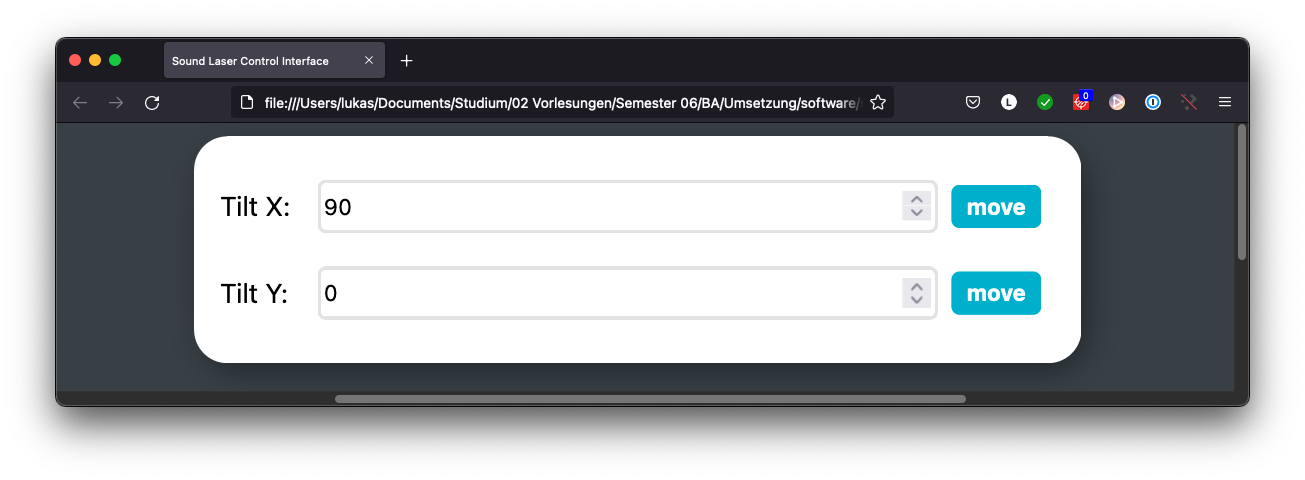
\includegraphics[height=\smallheight]{src/assets/pictures/software/control_interface_xl.png}
  \caption{Graphical control interface of the speaker}\label{fig:software:mov:website}
\end{figure}